\PassOptionsToPackage{unicode}{hyperref}
\PassOptionsToPackage{hyphens}{url}
%
\documentclass[12pt, a4paper]{article}
\usepackage[a4paper,margin=3cm]{geometry}
\setlength\parindent{0pt}
\setlength\parskip{6pt}
\usepackage{mathptmx}
\usepackage{amsmath,amssymb}
\usepackage[T1]{fontenc}
\usepackage[utf8]{inputenc}
\usepackage{textcomp}
\usepackage{graphicx}
\usepackage{booktabs}
\usepackage[font=small,labelfont=bf]{caption}
\usepackage[hidelinks]{hyperref}

\author{Zahra Amani Aghbolagh, MSc Artificial Intelligence, 0001208786
\\Seyeddanial Azimi, MSc Artificial Intelligence, 0001208680
\\Farzam Manafzadeh, MSc Artificial Intelligence, 0001248116
\\Kianaz Narehei, MSc Artificial Intelligence, 0001208574}
\date{}
\title{Structural Resilience and Hub Dependence\\in US Airline Networks}

\begin{document}
\maketitle

%=====================================================================
\section{Introduction}
\label{introduction}

This project applies network analysis to transport, specifically to the structure of
airline route networks. A route network determines which journeys are possible. If an
airline concentrates its routes on a few hubs, passengers can reach many destinations
with one connection, but most of those connections pass through the same airports.
When such a hub closes because of weather, a strike or an IT failure, the effect
reaches far beyond its own flights. Network science studies this trade-off by removing
airports from the network and measuring how much connectivity remains
\cite{albert2000,holme2002}.

We study three large US carriers in the second quarter of 2025: American Airlines
(AA), Delta Air Lines (DL) and Southwest Airlines (WN). AA and DL run classic
hub-and-spoke systems, while WN is known for a more point-to-point network. Using 2007
data, Wuellner et al.\ found that Southwest's network withstood targeted attacks better
than those of the hub carriers and linked this to its large $k$-core
\cite{wuellner2010}. More generally, networks with heavy-tailed degree distributions
tolerate random failures but break apart quickly when hubs are removed
\cite{albert2000}. The world air network has been described as a dense core with a
fragile, star-like periphery \cite{verma2014}, and it shows a clear community
structure \cite{guimera2005}.

Several earlier results shaped our design. Holme et al.\ \cite{holme2002} found that
recalculating the attack ranking after each removal is usually more harmful than ranking once. Newman \cite{newman2002} showed that assortative networks, in which hubs link
to other hubs, are more robust to the removal of vertices. For community-based
measures, Good et al.\ \cite{good2010} showed that modularity maximisation usually
admits many different near-optimal partitions, so measures built on one partition
need to be treated with care.

%=====================================================================
\section{Problem and Motivation}
\label{problem-and-motivation}

We ask two research questions. \textbf{RQ1}: how does the organisation of each
network relate to its structural resilience when airports are removed, and does the
observed resilience differ from what the airports' degrees alone would produce?
\textbf{RQ2}: which airport-level measures identify the airports whose individual
removal causes the largest loss? From these questions we derived three hypotheses and
fixed their decision rules before running the main experiments.

\begin{itemize}
\item \textbf{H1}: removing airports in order of degree or betweenness causes more
damage than removing the same number of airports at random.
\item \textbf{H2}: observed resilience differs systematically from that of random
networks with the same degrees.
\item \textbf{H3}: airports whose routes span more communities cause larger losses
than airports of similar degree.
\end{itemize}

Answering these questions has practical value. Hub closures are recurring events,
caused by storms, air-traffic restrictions or IT outages, and when one happens the
airline has to decide which connections it can still offer. Airlines, airports and
regulators therefore need to know which closures would disconnect large parts of the domestic network and
whether some carriers are structurally more exposed than others. Comparing AA and DL
with WN also speaks to the choice between hub-and-spoke and point-to-point models,
which trade convenient connections against exposure to a few critical airports.
There is also an open
methodological point. It is not obvious whether resilience depends on how routes are
\emph{arranged} or only on how many routes each airport has, and degree-preserving
null models \cite{maslov2002} allow the two to be separated. A related question is
whether ``bridging'' airports, which connect different regional communities, matter
more than their size suggests \cite{guimera2005b}.

The project makes three contributions. First, it gives an updated comparison of hub
dependence in three major US networks and traces the AA/DL versus WN contrast to one
simple feature, the number of small airports that depend on a single hub. Second, it
shows that the usual comparison with degree-preserving null models has little power
for hub-and-spoke networks under targeted removal, because real and randomised
networks both reach an efficiency floor after a handful of removals. Third, it finds
that community participation adds little to degree when predicting the impact of
single airports.

%=====================================================================
\section{Datasets}
\label{datasets}

\textbf{Source.} We use the publicly available \emph{Marketing Carrier On-Time
Performance} files of the US Bureau of Transportation Statistics (BTS) for April,
May and June 2025 \cite{bts}. The data were already in digital form, so no
digitisation was needed. We downloaded the three monthly CSV files, which together
contain 1,985,849 flight records. Keeping AA, DL and WN as marketing carriers leaves
1,292,785 scheduled flights, including those operated by regional partners under these
brands. Checks found no duplicate records, self-loops or routes created only by
diverted flights. Cancelled flights (2.3\%,
1.1\% and 0.5\% for AA, DL and WN) were kept because they were part of the published
schedule.

\textbf{Networks.} We analyse \textbf{three monomodal (one-mode) networks}, one per
airline. All three are built in the same way, so the same set of measures can be
applied to each and the results compared. \emph{Nodes} are airports, identified by BTS
airport ID. A \emph{directed edge} (arc) from airport $i$ to airport $j$ exists if at
least one nonstop flight from $i$ to $j$ was scheduled during the quarter. Each arc
carries the number of scheduled flights as a weight. We use the weight only for
description, and all resilience experiments treat routes as present or absent. All
three networks turned out to be fully reciprocal (every route has a return route) and
strongly connected. Degree, clustering, transitivity, assortativity, $k$-cores and
communities are computed on the undirected binary projection, in which $i$ and $j$
are linked if they share a route. Because of reciprocity, the projection loses no
information. Path-based measures (betweenness, efficiency, reachability and
components) use the directed network.

\textbf{Tools.} Data were stored as CSV files and handled with Python (pandas, NumPy).
Network measures were computed with NetworkX \cite{networkx} and statistics with SciPy
and scikit-learn. The analysis consists of eight Jupyter notebooks run in a pinned
software environment. Data, code, result tables and figures are available in the
project repository \cite{repo}.

%=====================================================================
\section{Validity and Reliability}
\label{validity-and-reliability}

\textbf{Validity.} Our model represents the structure of each airline's network. A
route exists if a single flight was scheduled in the quarter, and frequencies, seat
capacity and passenger flows do not enter the removal experiments. Removing an airport
deletes all its routes, with no rerouting, extra flights or recovery, so efficiency
loss is lost access in the route map and says nothing directly about stranded
passengers or economic cost. The quarterly network also merges routes
that may run at different times, so a path in it is a possible connection that may
not correspond to a bookable itinerary. To check that this aggregation does not drive
the results, we rebuilt the networks for each month separately and for routes with at
least 13 flights in the quarter, roughly a weekly service. The airline contrast held in both checks.
Under degree targeting, $K_{50}$ (Section~\ref{sec:h1}) stayed at 3 for AA and DL and
at 9 or 10 for WN.
Finally, three airlines in one quarter are case studies and do
not form a sample. The three networks also differ in size and density at the same
time, which limits how far their differences can be attributed to network design
alone.

\textbf{Reliability.} Every random step (Louvain runs, null networks, removal
orders and bootstrap samples) is seeded and recorded. The H1 verdicts did not change in 100 replicates with randomly broken ties. A second,
independent implementation starting from the raw files reproduced all values to
floating-point precision, and permutation $p$-values up to Monte Carlo error. With identical seeds, Louvain gives different partitions in
different NetworkX versions (17, 34 and 14 of 100 runs changed between versions 3.6.1
and 3.7). This moved participation-based values only in the second or third
decimal and changed no verdict, but it is why we pinned all package versions. The null
intervals also have limited precision. Between 150 and 200 null networks, the
endpoints of 7.6\% of the diagnostic cells moved by more than 10\% of the interval
width, so results close to an interval boundary should be read with caution. Finally,
the swap chains start from the observed network, and we cannot prove that they sample
uniformly from all graphs with the same degrees \cite{fosdick2018}.

%=====================================================================
\section{Measures and Results}
\label{measures}

Each subsection names the phenomenon studied, the measure used and its meaning for an
airline network, and then reports the results. Table~\ref{tab:struct} summarises the descriptive
measures.

\begin{table}[t]
\centering
\caption{Structure of the three networks (April--June 2025). Path length and
efficiency use the directed network; all other measures use the undirected projection.}
\label{tab:struct}
\small
\setlength\tabcolsep{4pt}
\begin{tabular}{p{6.4cm}rrr}
\toprule
Measure & AA & DL & WN \\
\midrule
Airports / directed routes & 230 / 1,808 & 212 / 1,506 & 104 / 1,792 \\
Density & 0.034 & 0.034 & 0.167 \\
Mean degree & 7.9 & 7.1 & 17.2 \\
Largest hub (share of airports reached) & DFW (79\%) & ATL (73\%) & DEN (83\%) \\
Airports with a single route partner & 55 (23.9\%) & 70 (33.0\%) & 2 (1.9\%) \\
Degree centralisation & 0.767 & 0.703 & 0.681 \\
Gini of scheduled departures & 0.732 & 0.738 & 0.617 \\
Average local clustering & 0.714 & 0.601 & 0.784 \\
Transitivity & 0.119 & 0.141 & 0.371 \\
Mean shortest path (flight legs) & 2.11 & 2.20 & 1.90 \\
Global efficiency & 0.492 & 0.478 & 0.572 \\
Degree assortativity & $-0.703$ & $-0.667$ & $-0.542$ \\
Innermost $k$-core (core number; share) & 11; 7.4\% & 12; 8.0\% & 15; 26.9\% \\
Best Louvain modularity $Q$ (100 runs) & 0.212 & 0.227 & 0.190 \\
Mean ARI between Louvain runs & 0.69 & 0.72 & 0.63 \\
\bottomrule
\end{tabular}
\end{table}

\subsection{Centrality, hub concentration and scale}

To see how strongly each airline depends on a few hubs, we use degree $k_i$, the
number of route partners of airport $i$ (in- and out-degree coincide), together with
the degree distribution, Freeman degree centralisation \cite{freeman1978} and the Gini
coefficient of departures. Degree counts the direct destinations an airport offers.
Centralisation equals 1 for a perfect star, so it shows how far a single hub dominates
the network, and the Gini coefficient shows how unequally flights are spread across
airports. To find the transfer junctions we use directed betweenness centrality, the
share of shortest paths that pass through an airport.

AA and DL are each dominated by one hub. DFW reaches 79\% of AA's airports and ATL
73\% of DL's, with centralisation of 0.77 and 0.70. Their degree distributions are
strongly right-skewed. A quarter of AA's airports and a third of DL's have exactly one
route partner, while a few hubs have more than 100. WN is also hub-concentrated
(centralisation 0.68), but its degrees are spread over a wide range and only 2
airports have a single partner. Its departures are also less concentrated (Gini 0.62).
The AA and DL distributions are heavy-tailed, as expected for hub-and-spoke systems,
but we do not claim that the networks are \emph{scale-free}. With only 104--230 nodes
and degrees capped at $N-1$, fitting a power law would not be meaningful. Degree and
betweenness agree closely for WN (Spearman 0.89) and less for AA and DL (0.64 and
0.68), so in the hub carriers an airport's size and its position on shortest paths are
less tightly linked.

\subsection{Clustering, small-worldness and triads}

We next test whether the networks are small worlds, that is, locally cohesive and
compact at the same time. Local clustering is the share of an airport's partners that
are themselves linked, that is, how often passengers can also fly directly between
an airport's destinations. Transitivity computes the same ratio over the whole network
and is dominated by the hubs. A small world combines clustering much higher than in a
random graph with comparably short paths, so we compare clustering and mean shortest
path with an Erd\H{o}s--R\'enyi benchmark and with the degree-preserving null networks
of Section~\ref{sec:h2}.

Average paths are short, between 1.9 and 2.2 legs. For AA and DL they are shorter than
the Erd\H{o}s--R\'enyi estimate $\ln N/\ln\langle k\rangle$ (2.64 and 2.73).
Clustering is far above the random-graph value, which equals the density (the share
of possible routes that actually exist). It is about
20 times higher for AA and DL (0.71 and 0.60 against 0.034) and about 5 times higher
for WN (0.78 against 0.167). By this standard all three networks are small worlds. The
degree-preserving reciprocal null networks, however, reach the same clustering (means
0.718, 0.621 and 0.776) and transitivity (0.122, 0.145 and 0.370), with path lengths
within 0.04 legs of the observed ones. The small-world property therefore follows from
the degree sequence itself. This also explains why local clustering is so much higher
than transitivity in AA and DL. Spokes served by two linked hubs have clustering 1,
while the hubs, whose partners are mostly unlinked, dominate transitivity. We did not run a directed triad census. Full
reciprocity makes every connected pair mutual, so triads reduce to the undirected
triangles that transitivity already counts.

\subsection{Assortativity and core--periphery}

To see whether hubs link mainly to other hubs or to small airports, we use degree
assortativity \cite{newman2002}, which measures homophily by
degree. It is the correlation between the degrees of linked airports. Positive values
mean that airports connect to airports of similar size, and negative values mean that
hubs mainly serve small airports. To look for a dense core we use the $k$-core decomposition.
The $k$-core is the largest set of airports in which each is linked to at least $k$
others in the set. The innermost core is the densely interconnected group of hubs, and
the airports outside it form the periphery.

All networks are strongly disassortative, as expected in hub-and-spoke systems, but WN
less so ($-0.54$ against $-0.70$ and $-0.67$). WN's innermost core holds 27\% of its
airports, compared with 7--8\% for AA and DL. Much of the AA and DL periphery depends
on the hubs, and 55 and 70 of their airports respectively have core number 1.

\subsection{Communities}

To find regional groups of airports we use Louvain modularity maximisation
\cite{blondel2008} at resolution 1, run with 100 seeds. Modularity $Q$ compares the
number of links inside groups with the number expected at random, and we measure the
agreement between runs with the adjusted Rand index (ARI). To identify airports that
bridge groups we compute the participation coefficient \cite{guimera2005b}
\begin{equation}
P_i = 1 - \sum_c \left(\frac{k_{ic}}{k_i}\right)^2,
\end{equation}
where $k_{ic}$ is the number of partners of $i$ in community $c$, and average it over
the 100 runs. $P_i$ is 0 when all of an airport's routes stay in one community and
approaches 1 when they are spread evenly, so airports with high $P_i$ act as bridges.

The communities we found are weak and unstable. The best modularity is only 0.21, 0.23
and 0.19, and the 100 runs give 100, 100 and 84 different partitions (mean ARI 0.69,
0.72 and 0.63). A typical airport's participation varies by 0.17--0.26 across runs.
This is the degeneracy of modularity described in Section~\ref{introduction}. Still, all observed values lie above the modularity range of the
reciprocal null networks ($[0.166, 0.176]$, $[0.199, 0.211]$ and $[0.115, 0.127]$),
so each airline groups its routes regionally more than its degrees require.
Participation is strongly correlated with degree (Spearman 0.72, 0.84 and 0.61).

\subsection{H1: connectedness under targeted and random removal}
\label{sec:h1}

To measure how fast connectivity degrades when airports fail, we remove airports by
degree, by betweenness (with rankings fixed on the intact network) or at random (100
recorded orders), at 5\%, 10\%, 15\% and 20\% of the airports. We measure damage with
directed global efficiency \cite{latora2001}
\begin{equation}
E = \frac{1}{N(N-1)} \sum_{i\neq j} \frac{1}{d_{ij}},
\end{equation}
where $d_{ij}$ is the number of legs on the shortest path from $i$ to $j$ and
unreachable pairs contribute zero. Efficiency captures how easily passengers can
travel between all pairs of airports. We also record reachability, the share of
ordered pairs that remain connected, which shows whether a journey is possible at all,
and the size of the largest strongly connected component (SCC), the largest group of
airports that can all reach each other. $N$ stays equal to the original number of
airports, so removed airports count as lost access. H1 holds for a strategy if the
targeted loss exceeds the 97.5th percentile of random losses for efficiency at all
four levels and for reachability and SCC at three or more. To compare the speed of
collapse, we also remove airports one at a time and record $K_{50}$, the number of
removed airports at which efficiency first falls to half its intact value.

\begin{figure}[t]
\centering
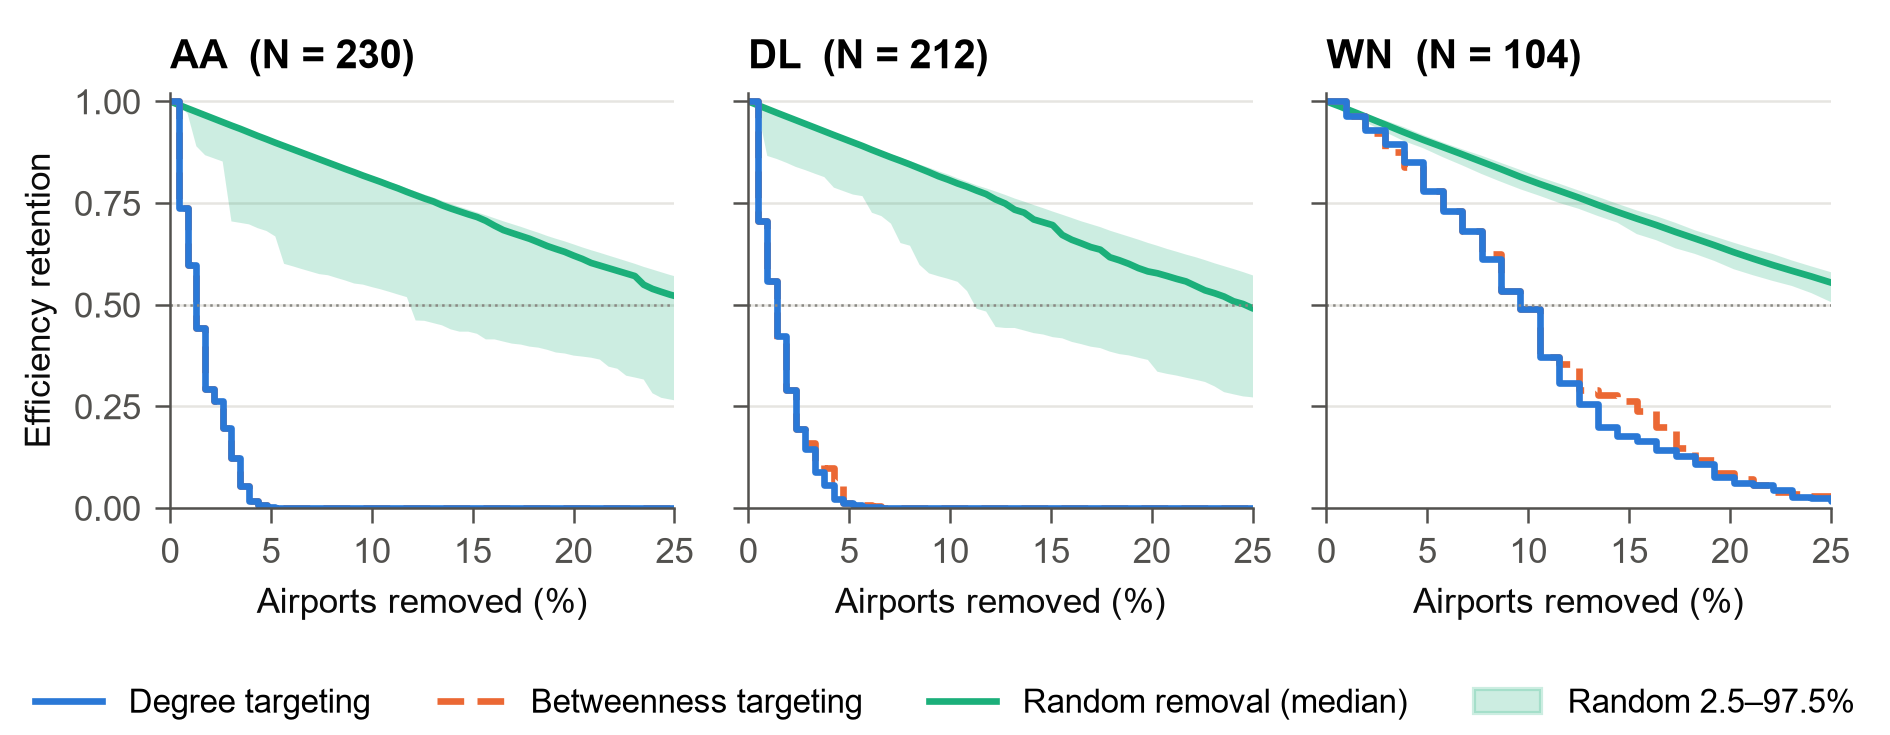
\includegraphics[width=\textwidth]{figures/fig1_retention_curves.png}
\caption{Efficiency retention as airports are removed one at a time by degree, by
betweenness, and in 100 random orders (band: 2.5th--97.5th percentiles). The dotted
line marks half of the intact efficiency.}
\label{fig:curves}
\end{figure}

\textbf{H1 is supported for all three airlines and both strategies.} Every targeted
loss exceeds the 97.5th percentile of random losses for all measures and levels. The
size of the gap, however, differs greatly between airlines (Figure~\ref{fig:curves}).
At 5\% removal, degree targeting leaves AA with 0.05\% of its efficiency and DL with
0.8\%, compared with 87\% and 88\% under random removal. WN keeps 78\% (90\% at random)
and degrades gradually. Removing only three airports halves the efficiency of AA and
DL ($K_{50}=3$), whereas WN needs ten. Under random removal the median $K_{50}$ is
60.5, 52.5 and 30 airports.

\begin{figure}[t]
\centering
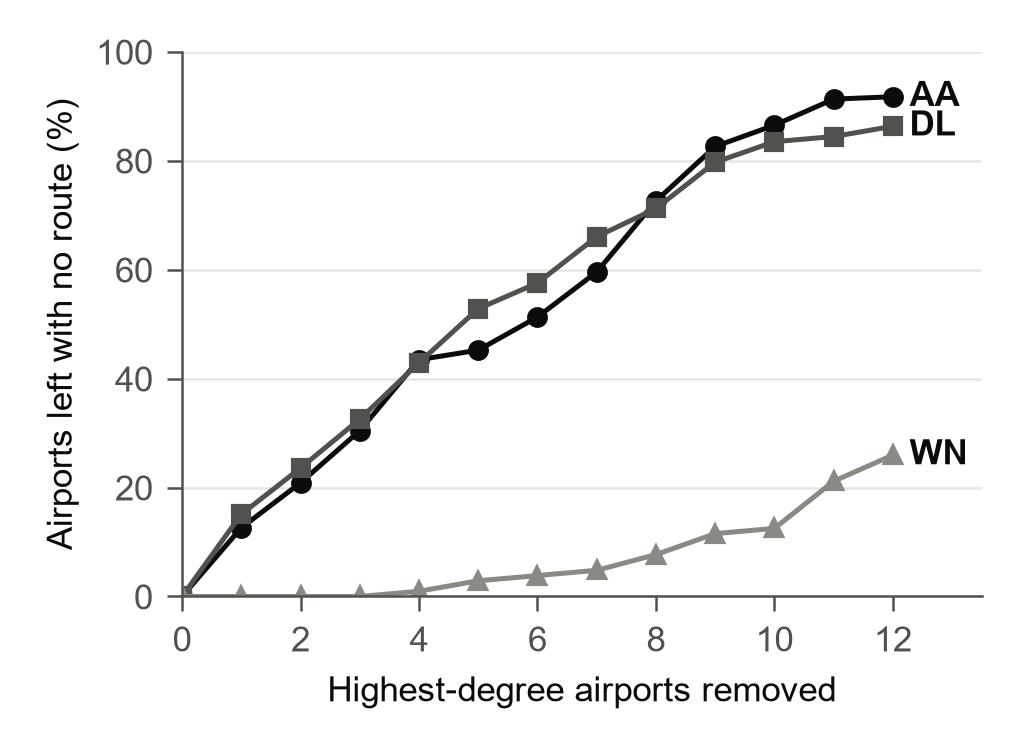
\includegraphics[width=0.6\textwidth]{figures/fig2_isolated_airports.png}
\caption{Share of airports left without any route after removing the $k$ airports with
the highest degree.}
\label{fig:captive}
\end{figure}

Figure~\ref{fig:captive} helps explain the difference. Removing DFW alone leaves 29 AA
airports with no route, and removing the top five hubs cuts off 104 airports (45\%).
For DL, the top four hubs cut off 91 (43\%). In WN, removing the top three airports
isolates none. The hubs themselves are densely linked, with 62 of the 66 possible
links among AA's 12 largest airports present. The collapse therefore comes from the
many small airports that are \emph{hub-captive}, meaning that all their partners are
among the removed hubs. Recomputing the rankings after every removal \cite{holme2002}
hardly changes the result ($K_{50}$ stays at 3, 3 and 10).

\subsection{H2: comparison with degree-preserving null models}
\label{sec:h2}

We then ask whether resilience depends on how routes are arranged or only on the
degrees. The primary null model rewires each network with directed two-edge swaps that
keep every in- and out-degree \cite{maslov2002}, giving 200 networks per airline. A
supplementary null of 100 networks swaps reciprocal route pairs and so also keeps full
reciprocity. These networks keep how many routes each airport has but randomise who
connects to whom, so a difference between them and the observed network points to the
arrangement of routes. An outcome deviates if it lies outside the 2.5th--97.5th
percentile interval of the null networks. A strategy deviates systematically if
efficiency does so in the same direction at three or more levels together with
reachability or SCC, and H2 holds if two of the three strategies deviate. As an
exploratory addition, we summarise the whole removal curve with a robustness score
adapted from \cite{schneider2011}, $R_E = \frac{1}{N}\sum_{q=1}^{N} E(q)/E_0$, the
mean efficiency retention over the full sequence of removals.

\begin{figure}[t]
\centering
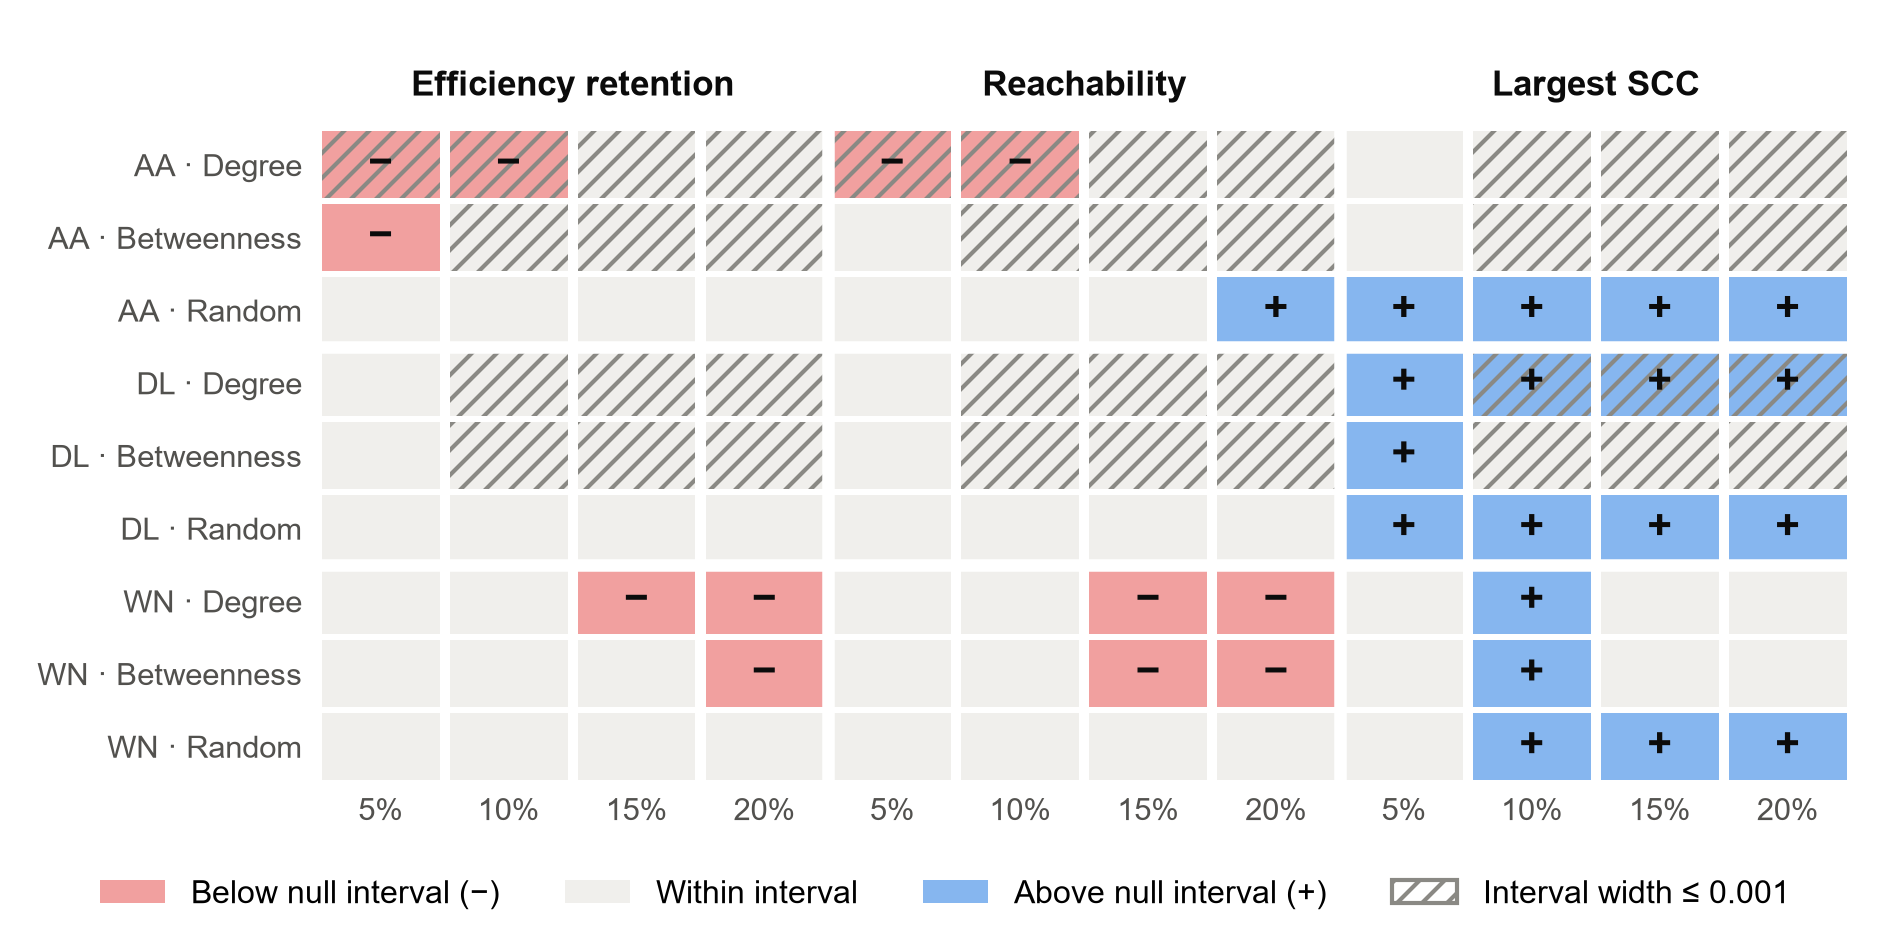
\includegraphics[width=\textwidth]{figures/fig3_h2_cells.png}
\caption{Position of each observed H2 outcome relative to the 2.5th--97.5th
percentile interval of the 200 primary null networks. Hatching marks intervals no
wider than 0.001.}
\label{fig:h2}
\end{figure}

\textbf{H2 is not supported for any airline.} Of the 108 decision cells, 77 lie inside
the null interval, 19 above it and 12 below it (Figure~\ref{fig:h2}). The null
networks are tightly constrained and still share 62--70\% of their routes with the
observed networks. In AA and DL, targeted removal drives observed and null networks
alike to almost zero efficiency by the 5\% level. Of their 48 targeted cells, 38 have
an interval no wider than 0.001, so the test has little power there. Most cells above
the interval concern the SCC under random removal and vanish against the reciprocal
null, so they probably reflect the reciprocity lost in the directed swaps. The full-curve score $R_E$ is less affected by this floor. For AA and DL it
lies inside both null ranges. For WN it is lower than in all 300 null networks under
both targeted strategies (0.094 under degree removal against 0.101--0.108), which
means that WN's real arrangement is slightly \emph{more fragile} than random
arrangements under sustained attack.

Within the reciprocal nulls, where all networks share the observed degrees,
resilience still varies with assortativity (exploratory; 378 Spearman tests per null
family, Benjamini--Yekutieli correction \cite{by2001}). Networks with less negative assortativity keep more early efficiency
under degree targeting in AA ($\rho = 0.52$) and DL ($\rho = 0.51$). These networks
also tend to have fewer hub-captive spokes ($\rho = -0.55$ and $-0.50$), an
association we have not shown to be causal. Modularity and the core measures show no association.

\subsection{H3: critical single airports}

Finally, we look at which airports cause the largest loss when they fail alone, and
whether bridging airports matter beyond their degree. For every airport with at least
two partners (175, 142 and 102 airports) we compute the efficiency loss $\Delta E_i$
of removing it alone. Because $N$ is fixed, this loss splits exactly into two parts,
\begin{equation}
\Delta E_i = \frac{H_i}{N(N-1)} + \frac{N-2}{N}\,D_i,
\end{equation}
where $H_i$, twice the harmonic centrality \cite{boldi2014}, is the lost access to and
from $i$, and $D_i$ (survivor damage) is the fall in efficiency among the other
airports. The first part describes how close $i$ is to the rest of the network. Only
the second part measures harm to other airports. Full support for H3 requires three
conditions: (i) a positive partial rank correlation between participation and loss
given degree, with a bootstrap interval above zero; (ii) a median out-of-bag gain of at
least 0.02 in rank-model $R^2$ when participation is added to degree, over 2,000
bootstrap samples; and (iii) higher loss for high-participation airports in two thirds
of the degree bins. Meeting one or two conditions gives partial support.

\begin{figure}[t]
\centering
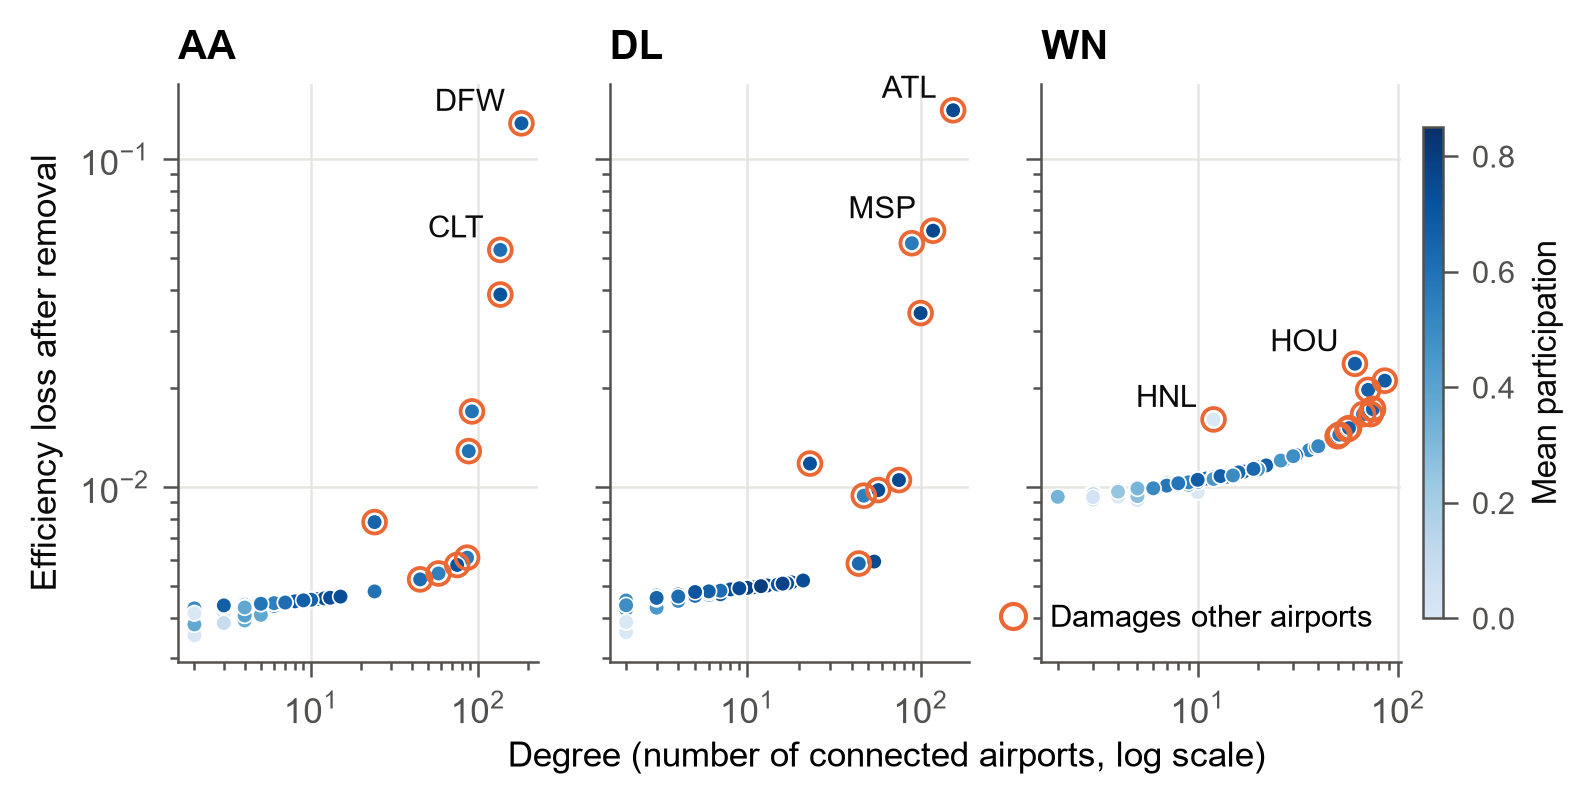
\includegraphics[width=0.85\textwidth]{figures/fig4_h3_loss_degree.png}
\caption{Efficiency loss from removing each airport against degree (log axes). Colour:
mean participation; rings: airports that also damage paths between other airports.}
\label{fig:h3}
\end{figure}

\begin{table}[t]
\centering
\caption{H3 evidence. Brackets: 2.5th--97.5th bootstrap percentiles.}
\label{tab:h3}
\footnotesize
\setlength\tabcolsep{3pt}
\begin{tabular}{p{4.4cm}ccc}
\toprule
 & AA & DL & WN \\
\midrule
Partial rank corr.\ (participation, loss $\mid$ degree) & 0.49 [0.37, 0.60] & 0.56 [0.41, 0.68] & 0.28 [$-0.07$, 0.55] \\
Median gain in $R^2$ & 0.040 [$-0.005$, 0.078] & 0.026 [$-0.002$, 0.050] & 0.003 [$-0.031$, 0.014] \\
Degree bins with higher loss & 7 of 7 & 7 of 8 & 6 of 8 \\
Conditions met / verdict & 2 of 3, partly & 2 of 3, partly & 1 of 3, partly \\
\bottomrule
\end{tabular}
\end{table}

Single-airport losses are highly concentrated. DFW alone removes 26\% of AA's
efficiency and ATL 29\% of DL's, while WN's most damaging airport, HOU, removes 4\%.
The own-access term accounts for 82\%, 77\% and 98\% of all loss. Only 10, 9 and 12
airports cause any survivor damage, and for the other 388 airports the loss is exactly
proportional to harmonic centrality. Degree and betweenness find 9--10 of the ten most
damaging airports, while participation finds only 0--5.
\textbf{H3 is partly supported for all three airlines} (Table~\ref{tab:h3}). In AA and DL, participation
has a clear positive partial correlation with loss and wins in most degree bins, but
no airline meets the prediction condition. Loss rises almost deterministically with
degree (Figure~\ref{fig:h3}), which leaves little for participation to explain. Part
of its association reflects links to larger airports. Adding mean neighbour degree as
a control lowers the partial correlation to 0.30 (AA), 0.43 (DL) and 0.06 (WN), and
with a flexible (spline) model of degree the cross-validated gain from participation
disappears. Honolulu harms others without bridging communities. Its participation is zero, yet it
causes WN's second-largest survivor damage because Hilo's only route goes there.

%=====================================================================
\section{Conclusion}
\label{conclusion}

All three networks fit the classic picture of attack vulnerability \cite{albert2000},
but they fail at different speeds. AA and DL are star-like hub systems, with a small
core and a large periphery of airports that depend on one or two hubs, similar to the
structure Verma et al.\ described for the world network \cite{verma2014}. WN has almost no single-route airports, a broader degree distribution and a
core holding a quarter of its airports, and it degrades gradually. With 2025 data and
a different damage measure, this confirms the ordering that Wuellner et al.\ found for
2007 \cite{wuellner2010}. Our results add a mechanism, since the difference follows
the number of hub-captive airports.

The null models show how much of this follows from the degrees alone. Random networks
with the same degrees closely reproduce the observed clustering and path length and,
for AA and DL, the observed resilience. The hub degrees are so large and the spoke
degrees so small that any arrangement leaves many airports dependent on the same few
hubs. Route arrangement has smaller effects, such as stronger regional modularity than in
random networks and WN's slightly greater fragility under sustained attack. Among degree-matched networks, less
disassortative ones resist hub loss better, in line with Newman's results on
assortative mixing \cite{newman2002}.

For single airports (RQ2), degree and betweenness identify the critical airports. For
almost all airports the loss consists only of their own lost access, which behaves
like a closeness measure and follows degree. Harm to other airports comes from a few
large airports and from isolated cases such as Honolulu. Community participation
describes a weaker property, how close an airport is to the network beyond what its
degree implies, and it is too unstable to serve as an indicator of criticality.

Within our structural model, these findings have a practical reading. The exposure
of AA and DL comes less from the hubs themselves, which are almost fully linked to
one another, than from the many spokes that rely on a single hub. This suggests,
although we did not test it, that giving some of these airports a second connection
would reduce exposure more than adding links between hubs. WN's risk is spread more evenly, and no single closure removes
more than 4\% of its efficiency, but its arrangement copes slightly worse than random
alternatives when disruption continues.

%=====================================================================
\section{Critique}
\label{critique}

We consider RQ1 largely answered. We can explain why the airlines differ, and we show
that for AA and DL resilience is essentially fixed by the degree sequence. The H2
test, however, did not work as intended for AA and DL. Comparing networks at fixed
removal fractions tells us little once all of them have reached the efficiency floor.
Removal levels set relative to each network's collapse point, or a full-curve score
such as $R_E$ as the pre-specified test, would have made the comparison more powerful.
RQ2 is answered for our efficiency measure, but the decomposition shows that
efficiency loss mostly measures an airport's own access. A measure focused on harm to
others, such as survivor damage or path redundancy, would capture criticality better.
Participation also depends on an unstable partition. A consensus partition or a method
based on a statistical model, such as a stochastic block model, would give H3 a firmer
basis.

With more data, we could weight routes by frequency or seats, use passenger
itineraries and model rerouting, which would turn structural loss into a measure of
operational impact. Including more airlines and quarters would allow conclusions
beyond three case studies. A null model that also preserves flight frequencies or
geography would show whether regional organisation shapes resilience beyond what
degree explains. Finally, because all three networks are fully reciprocal, the
directed analysis adds little to the undirected one, and flight frequencies never
enter the resilience measures. Weighted versions of efficiency and betweenness
would show whether frequency changes which airports are critical.

%=====================================================================
\small
\begin{thebibliography}{99}
\bibitem{albert2000} Albert, R., Jeong, H.\ and Barab\'asi, A.-L. (2000). Error and attack tolerance of complex networks. \emph{Nature}, 406, 378--382.
\bibitem{holme2002} Holme, P., Kim, B.\ J., Yoon, C.\ N.\ and Han, S.\ K. (2002). Attack vulnerability of complex networks. \emph{Physical Review E}, 65, 056109.
\bibitem{wuellner2010} Wuellner, D.\ R., Roy, S.\ and D'Souza, R.\ M. (2010). Resilience and rewiring of the passenger airline networks in the United States. \emph{Physical Review E}, 82, 056101.
\bibitem{verma2014} Verma, T., Ara\'ujo, N.\ A.\ M.\ and Herrmann, H.\ J. (2014). Revealing the structure of the world airline network. \emph{Scientific Reports}, 4, 5638.
\bibitem{guimera2005} Guimer\`a, R., Mossa, S., Turtschi, A.\ and Amaral, L.\ A.\ N. (2005). The worldwide air transportation network. \emph{PNAS}, 102(22), 7794--7799.
\bibitem{maslov2002} Maslov, S.\ and Sneppen, K. (2002). Specificity and stability in topology of protein networks. \emph{Science}, 296, 910--913.
\bibitem{guimera2005b} Guimer\`a, R.\ and Amaral, L.\ A.\ N. (2005). Functional cartography of complex metabolic networks. \emph{Nature}, 433, 895--900.
\bibitem{bts} US Bureau of Transportation Statistics. Marketing Carrier On-Time Performance (Beginning January 2018), April--June 2025. \url{https://transtats.bts.gov}
\bibitem{networkx} Hagberg, A.\ A., Schult, D.\ A.\ and Swart, P.\ J. (2008). Exploring network structure, dynamics, and function using NetworkX. \emph{Proc.\ SciPy 2008}, 11--15.
\bibitem{repo} Project repository (notebooks, data, results, verification scripts). \url{https://github.com/zahraamani7065/airline-network-resilience}
\bibitem{fosdick2018} Fosdick, B.\ K., Larremore, D.\ B., Nishimura, J.\ and Ugander, J. (2018). Configuring random graph models with fixed degree sequences. \emph{SIAM Review}, 60(2), 315--355.
\bibitem{freeman1978} Freeman, L.\ C. (1978). Centrality in social networks: conceptual clarification. \emph{Social Networks}, 1(3), 215--239.
\bibitem{newman2002} Newman, M.\ E.\ J. (2002). Assortative mixing in networks. \emph{Physical Review Letters}, 89, 208701.
\bibitem{blondel2008} Blondel, V.\ D., Guillaume, J.-L., Lambiotte, R.\ and Lefebvre, E. (2008). Fast unfolding of communities in large networks. \emph{J.\ Stat.\ Mech.}, P10008.
\bibitem{good2010} Good, B.\ H., de Montjoye, Y.-A.\ and Clauset, A. (2010). Performance of modularity maximization in practical contexts. \emph{Physical Review E}, 81, 046106.
\bibitem{latora2001} Latora, V.\ and Marchiori, M. (2001). Efficient behavior of small-world networks. \emph{Physical Review Letters}, 87, 198701.
\bibitem{schneider2011} Schneider, C.\ M., Moreira, A.\ A., Andrade, J.\ S., Havlin, S.\ and Herrmann, H.\ J. (2011). Mitigation of malicious attacks on networks. \emph{PNAS}, 108(10), 3838--3841.
\bibitem{by2001} Benjamini, Y.\ and Yekutieli, D. (2001). The control of the false discovery rate in multiple testing under dependency. \emph{Annals of Statistics}, 29(4), 1165--1188.
\bibitem{boldi2014} Boldi, P.\ and Vigna, S. (2014). Axioms for centrality. \emph{Internet Mathematics}, 10, 222--262.
\end{thebibliography}

\end{document}
